\documentclass[10pt,english]{article}
\usepackage[T1]{fontenc}
\usepackage[latin9]{inputenc}
\usepackage[a4paper]{geometry}
\geometry{verbose}
\pagestyle{plain}
\usepackage{babel}
\usepackage{graphicx}

\usepackage{amsmath}
\usepackage{setspace}
\onehalfspacing
\usepackage[unicode=true, pdfusetitle,
 bookmarks=true,bookmarksnumbered=false,bookmarksopen=false,
 breaklinks=false,pdfborder={0 0 1},backref=false,colorlinks=false]
 {hyperref}

%\usepackage{ccfonts,eulervm}
\usepackage{fouriernc}
\usepackage{siunitx}
\usepackage{microtype}
\usepackage{nicefrac}
\usepackage{subfigure}

\begin{document}

\title{Michaelmas Term Summary}
\author{Gen Zhang}

\maketitle

\section{Very briefly}

Data analysed: ear, both B and B+S with genetic labelling and B+S with EdU labelling; oesophagus, B and B+S with genetic labelling only. The basal-only data (B) consists of long time statistics, up to one year after labelling. The basal and suprabasal data (B+S) consists only of short time statistics, on the order of a few divisions after labelling.
The pulsed EdU labelling shows significant clustering of labelled individuals/pairs, and confidence of resolving separate clones is low after just a couple of rounds of division.

Bayesian methods were used to analyse the data.

Conclusions: the scaling limit at large $t$ is well verified, and clearly exhibited by all basal data; the shorter time data show deviations from the purely stochastic model with parameters chosen to be consistent with the scaling behaviour. Synchrony/non-Markovian behaviour is suspected to be the culprit.

\section{The models}

The simplest model known to be in the universality class consistent with experiment is a purely stochastic fate choice model, where we distinguish between three types of cells. $A$ is a proliferating cell in the basal layer, capable of further division; $B$ is a differentiated cell in the basal layer, unable to divide further; and $C$ is a suprabasal cell. The choice of cell division/differentiation/stratification is assumed to be independent of cell age and lineage, i.e. purely Markovian.

\begin{align*}
A &\overset{\lambda}{\longmapsto} \begin{cases}
AA & r \\
AB & 1-2r \\
BB & r\end{cases} & B &\overset{\gamma}{\longmapsto} C
\end{align*}

If only the basal layer is important, then it is possible to simply not track $C$ cells, and have the replacement rule \[B \overset{\gamma}{\longmapsto} \emptyset.\]

\subsection{Numerical evaluation}

As long as the dynamics is Markovian, it is possible to write a master equation for the time evolution. It is set of first order coupled differential equations, of the form \[\dot{\mathbf P} = \mathbf T \mathbf P,\] where $\mathbf P$ is a infinite dimensional vector.

For the $ABC$ model, a crucial insight is that the total number of cells is a monotonic function. As such, the transition matrix $\mathbf T$ assumes a particular triangular form. This means that if we only care about clones up to a size $k$, we are free to truncate $\mathbf P$, and end up with a finite number of coupled equations to solve. In this case, the solution is simple, and can be formally given as \[\mathbf P = \exp\left(\mathbf T t\right)\mathbf P_0.\] Utilising the sparsity in $\mathbf T$, this allows rapid and numerically stable evaluation of $\mathbf P$ for any parameter $\left(\lambda, r, \gamma\right)$ at any time.

For the reduced $AB$ model, the finite cutoff is no longer accurate as the equations are arbitrarily coupled. For an initial condition of one type $A$ cell at $t=0$, the probability distribution $\mathbf P$ evolves diffusively, and in principle as long as the cutoff $k_\textrm{max} \gg \lambda t$ the error is not too great. However, in practice, the required safety margin is large and it is difficult if not impossible to give global error bounds --- it is unclear how the cutoff, which acts as a boundary condition, causes reflections in the diffusion which may propagate back. Instead, a method based around generating functions and discrete Fourier transforms was used.

Using $m$ and $n$ to denote the number of $A$ and $B$ cells in a clone, respectively, it is possible to write down the relevant master equation:
\begin{equation*}
\begin{split}
\frac{dP_{m,n}}{dt} &= \lambda\left[r(m-1)P_{m-1,n} + (1-2r)mP_{m,n-1} + r(m+1)P_{m+1,n-2}\right] \\ &+ \gamma (n+1) P_{m,n+1} \\ &- (\lambda m + \gamma n) P_{m,n}.
\end{split}
\end{equation*}

Casting this into the form of a generating function \[F(x,y,t) = \sum x^m y^n P_{m,n}(t),\] we obtain a partial differential equation for $F$:
\begin{equation*}
F_t = \lambda \left[r x^2 F_x + (1-2r) x y F_x + r y^2 F_x\right] + \gamma F_y - (\lambda x F_x + \gamma y F_y).
\end{equation*}

The characteristic curves are then given by:
\begin{align*}
\frac{dF}{ds}&=0 & \frac{d\tau}{ds}&=1 \\
\frac{d\xi}{ds}&= \lambda\left[\xi(1-\psi) - r(\xi - \psi)^2\right] & \frac{d\psi}{ds}&= \gamma(\psi-1)
\end{align*}

The initial conditions translate into
\begin{align*}
F(x,y,t=0) &= x & \xi(s=t) &= x & \psi(s=t) &= y
\end{align*}
and so
\begin{equation*}
F\left(x,y,t\right) = F\left(\xi(s=0), \psi(s=0), 0\right) = \xi(s=0).
\end{equation*}

Thus we have turned the problem into one involving an ordinary differential equation. This may be further simplified through a series of substitutions. First, \[\psi(s) = \left(y - 1\right)e^{\gamma(s-t)}+1,\] allowing the elimination of $s$: \[\frac{d\xi}{ds} = \frac{d\psi}{ds} \frac{d\xi}{d\psi} = \gamma \left(\psi - 1\right) \frac{d\xi}{d\psi} = \lambda\left[\xi(1-\psi) - r(\xi - \psi)^2\right].\] Finally, defining $u = 1-\psi = (1-y)e^{\gamma(s-t)}$ we can write \[\gamma u \xi^\prime = \lambda \left[\xi u - r\left(\xi + u - 1\right)^2\right],\] where the prime is differentiation with respect to $u$. The generating function is then \[F(x,y,t) = \xi\left(u = (1-y)e^{-\gamma t}\right).\]

At the end, we will be interested in the clone counts, which will be given by the generating function $G(z,t) = F(z,z,t)$. Specifically, the probability of a clone of size $k$ will be given by the appropriate coefficient in the Taylor expansion of $G$, which may be extracted by \[P_k(t) = \frac{1}{2\pi i}\oint_C \frac{G(z,t)}{z^{k+1}} dz,\] where the contour $C$ goes counterclockwise around the origin in the complex $z$ plane, within the radius of convergence of $G$. Since we know that $G(z,t)$ must be well-defined by its Taylor series expansion on the real interval $[0,1]$, the radius of convergence must be at least 1. Thus it would be sufficient to take C to be the unit circle.

The Cauchy integral may be approximated by a sum \[P_k(t) \approx \frac{1}{N} \sum_{j=0}^{N-1} G\left(e^{2\pi i j/N},t\right) e^{-2\pi i j k /N}\] which is the discrete Fourier transform. Thus evaluation of $G$ around the unit circle $N$ times would yield the first $N$ elements of $P_k$. The evaluation of $G$ may proceed via the differential equation for $\xi$, and dominates the time taken to calculate $P_k$. Thus in the interests of efficiency and error control, $N$ should be adaptively increased (through a series of doublings) until the global error (for the elements $P_k$ of interest) falls below an acceptable threshold. It is possible to get the first $O(100)$ elements of $P_k$ at $\lambda t \approx 50$ in around $\SI{10}{s}$.

\subsection{Scaling behaviour}

At sufficiently long times, we find that the clones exhibit a neat scaling behaviour \[k P^{>0}_k(k t) = \frac{\tau}{t}\exp\left(-\frac{\tau}{t}\right)\] where $\tau = \frac{\rho}{r\lambda}$ and \[P^{>0}_k = \frac{P_k}{1-P_0}.\] Note that although technically the un-conditional distribution also has a scaling behaviour \[k^2 P_k(k t) = \left(\nicefrac{\tau}{\rho t}\right)^2\exp\left(-\frac{\tau}{t}\right),\] this is not actually observable since experiments can only count the \emph{surviving} clones. On the other hand, this scaling behaviour is not single parameter, and would allow estimates of both $r\lambda$ and $\rho$ from the large $t$ statistics.

\section{Of Bayes and Men}

Given the ability to calculate $P_k$ at will, it is then a small matter to obtain estimates for the parameters of the model from data. For convenience in comparison with experiment, we replace the stratification rate $\gamma$ with the dimensionless quantity \[\rho = \frac{\lambda}{\lambda - \gamma}\] which gives the proportion of proliferating ($A$) cells in the basal layer at equilibrium. So for a given data $D$ and parameters $\theta$ we have, quite elementarily, \[p(\theta|D) = \frac{p(D|\theta)}{p(D)} p(\theta).\] Happily, $p(D|\theta)$ is, as discussed above, efficiently obtainable and $p(D)$ acts as just a normalisation constant in order that the left hand side is a proper probability distribution. In theory the prior $p(\theta)$ might be quite complicated, but in practice the data $D$ is sufficiently large (usually a few tens to a couple hundred clones) that variations to the prior is largely wiped out in the posteri distribution. For example, a uniform prior for $\lambda$ and a log-uniform prior both give the same posteri distribution to within numerical error. As such, uniform priors were used for simplicity. 

The posteri distribution $p(\theta|D)$ is a distribution over the three-dimensional space $(\lambda, r, \rho)$, which makes the full distribution rather difficult to visualise. Figure \ref{fig:ear_eyp_bs_3d} shows a typical distribution for a B+S dataset. A similar plot is possible for a basal layer only data set, which would show instead a hyperbolic sheet, concentrated around the timescale $\tau$, as the basal layer data tends to be collected for large $\lambda t$, at which point we enter into the scaling regime.

\begin{figure}[htb]
	\centering
	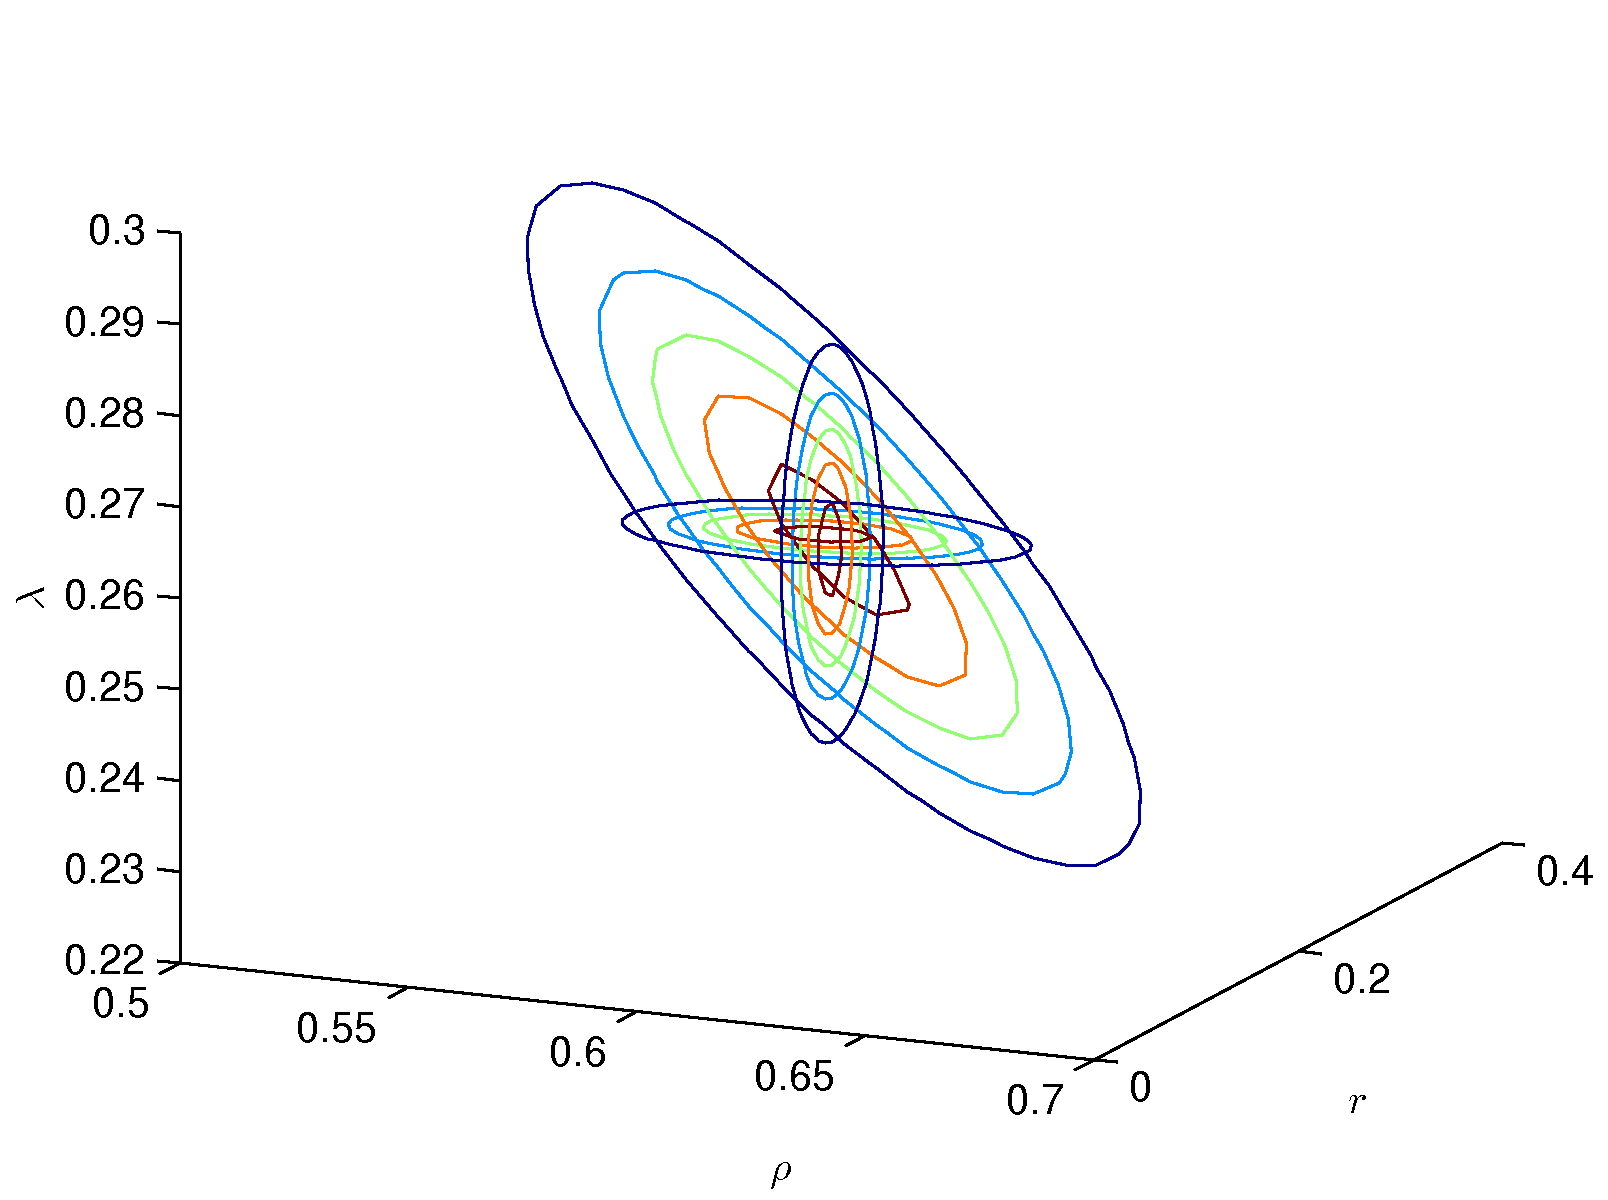
\includegraphics[width=0.9\textwidth]{ABC/ear_eyp_bs.png}
	\caption{\label{fig:ear_eyp_bs_3d}Posteri distribution for parameters of ear B+S data, at $3$ and $6$ weeks. The three sets of contours are sliced parallel to the axes, through the mean parameter $(\lambda, r, \rho) = (0.26 \pm 0.02~\textrm{/week}^{-1}, 0.25 \pm 0.03, 0.59 \pm 0.4).$ The contour lines are equal-spaced. The overall blob is extremely close to being Gaussian, with principal axes not aligned to the parameter space. The dataset consisted of $240$ clones sampled at $6$ weeks.}
\end{figure}

If we do not trust $\rho$ as measured from Ki67 and Ki86 expression rates, then the long term basal data cannot yield much beyond a value for $\tau$. In particular, it is not possible to extract $\lambda$, $r$ and $\rho$ independently. The data can still reveal a distribution for $\tau$, e.g. figure \ref{fig:ear_eyp_b_tau}. Nevertheless, this means that the most reliable estimate for $\lambda$ is from the short-time B+S data, where available.

\begin{figure}[htb]
	\centering
	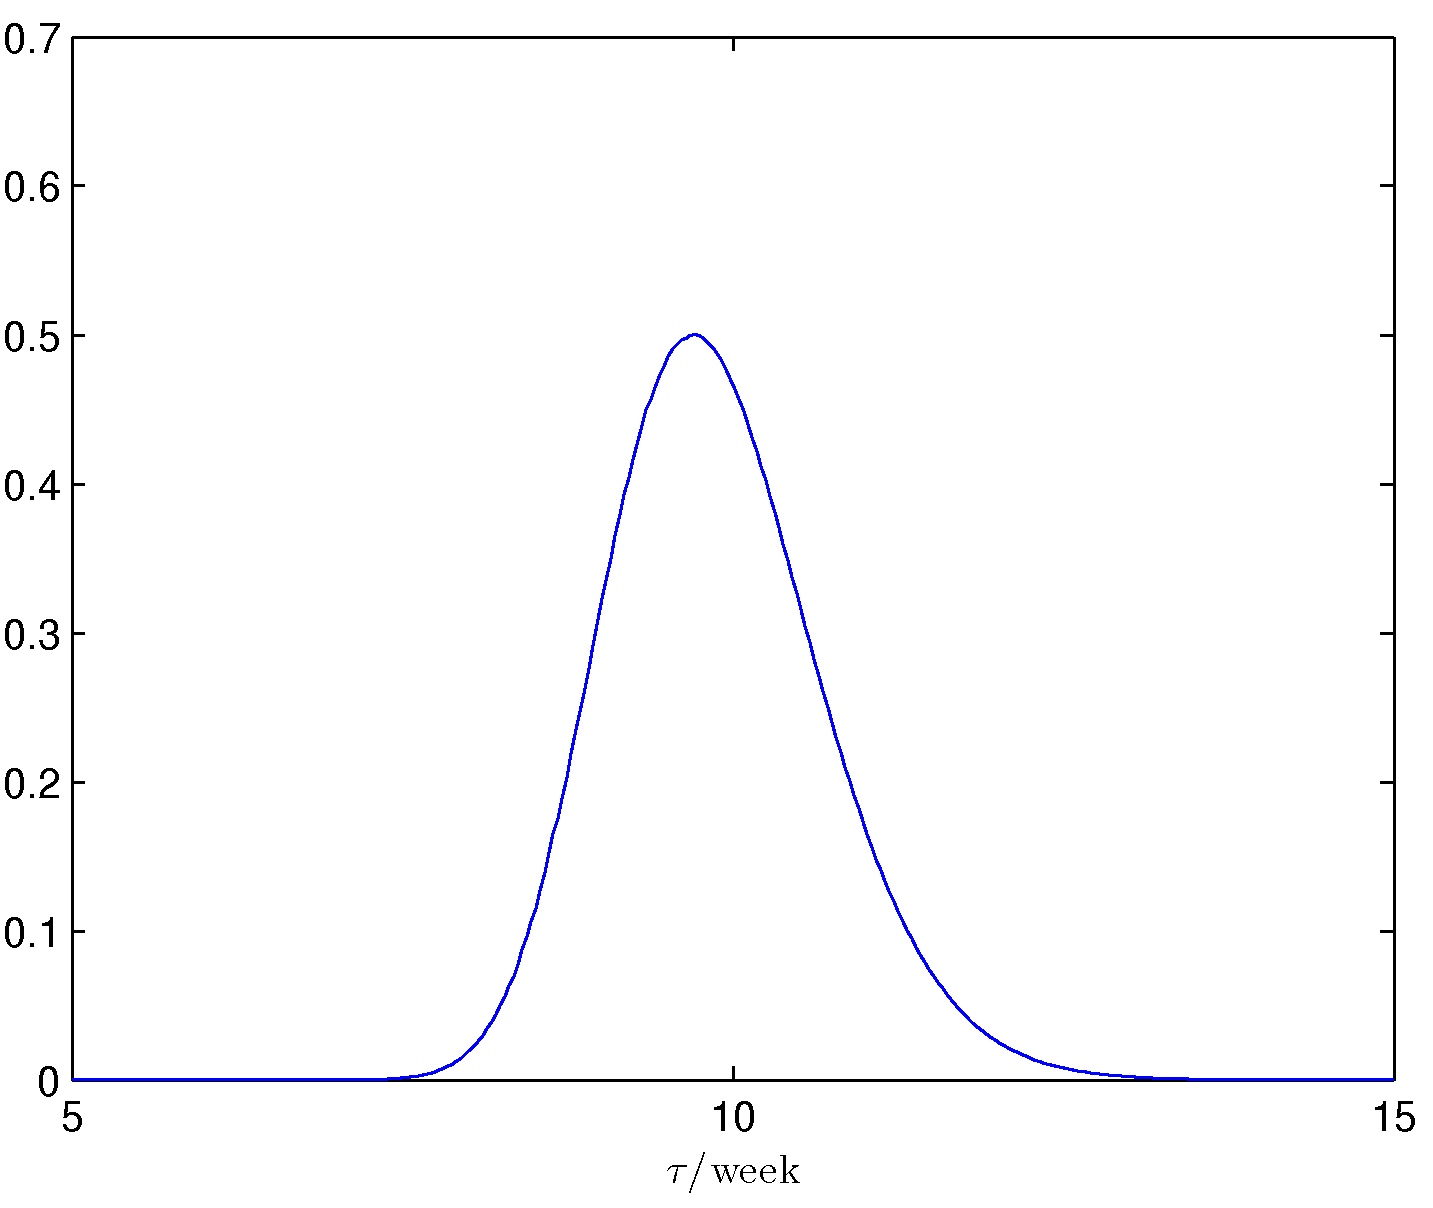
\includegraphics[width=0.8\textwidth]{AB/ear-eyp-b-tau.png}
	\caption{\label{fig:ear_eyp_b_tau}Posteri distribution for $\tau = \rho/r\lambda$ for ear basal data, out to one year. The distribution is fairly exactly log-normal, with $\tau = 10.3 \pm 0.9~\textrm{weeks}$. Rather gratifyingly, the posteri distribution knows something of the scale-free nature of the parameter even though the prior did not respect the symmetry.}
\end{figure}

As such, a reasonable protocol seems to be to use B+S data where possible to find a distribution for $\lambda$, and use that to inform the basal-only analysis, i.e. marginalise over $\lambda$. Doing so, we can put all the data together and find the total Bayesian inference using all the data. Figure \ref{fig:ear-eyp-combined} shows this for the ear.

\begin{figure}[htb]
	\centering
	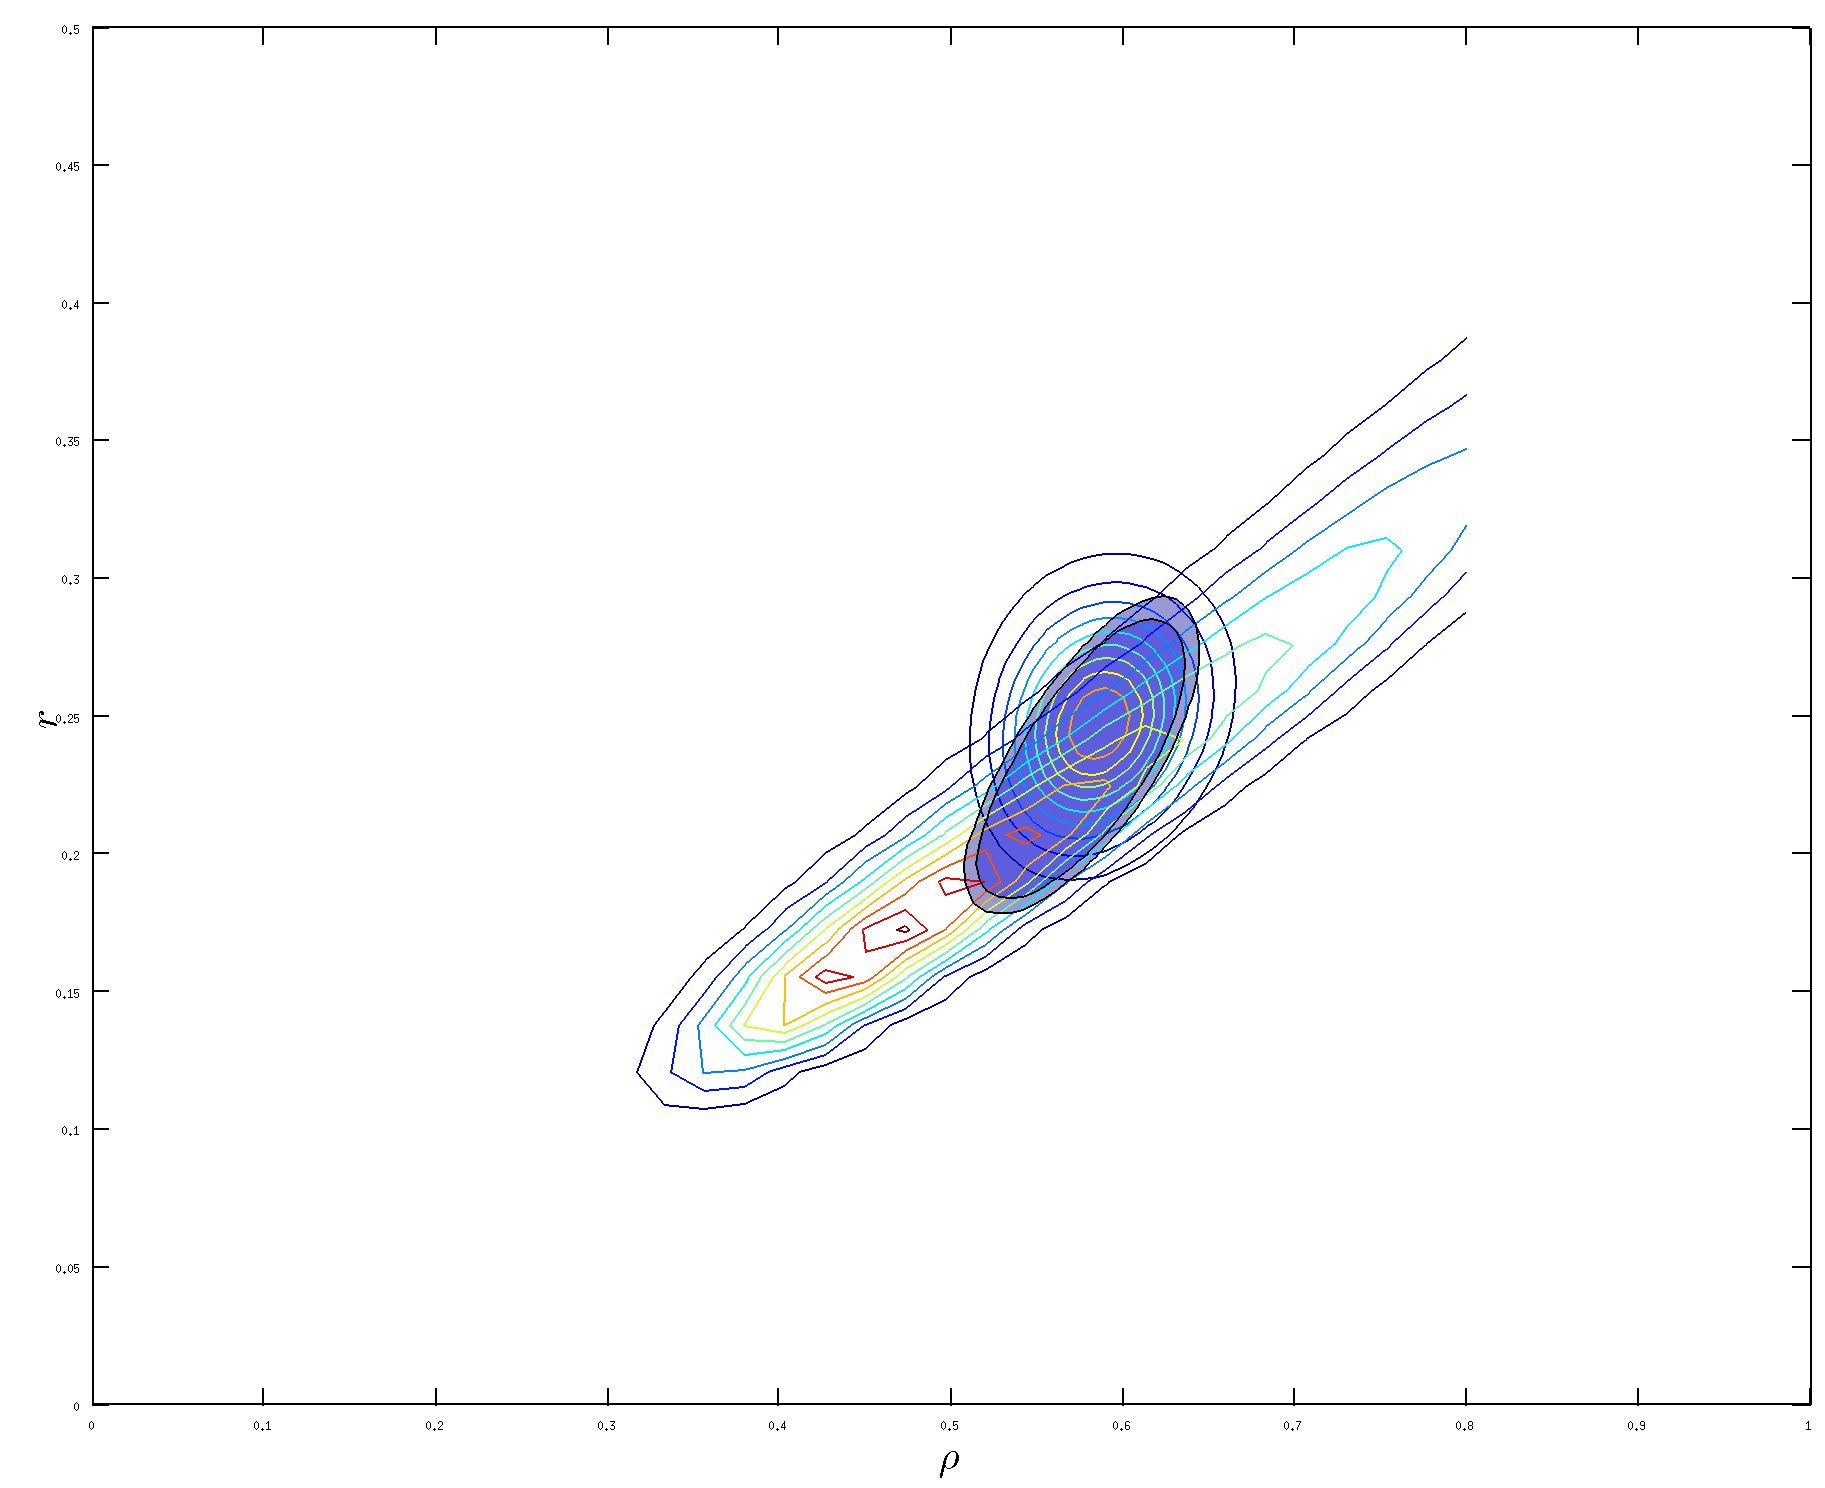
\includegraphics[width=0.8\textwidth]{ear-combined-projected-lambda.png}
	\caption{\label{fig:ear-eyp-combined}Super-imposed B+S and B data, marginalised over $\lambda$. The set of concentric circles show the B+S inference, successive rings enclosing extra $10\%$ of the probability, i.e. the outer ring shows the $90\%$ confidence region. The shaded regions correspond to the combined inference, using both B+S and long time basal-only data, and show the $90\%$ and $95\%$ confidence regions. Note that the special point $r=1/4$, $\rho=1/2$ is actually excluded.}
\end{figure}

\section{Still to do}

As of writing this, the oesophagus data has also pulled through, but with resolution issues --- I need to re-run the data to get nicer graphs. A more serious issue of estimating $\tau$ from the AB data has appeared however. It seems that a failure to sample adequetely over the entire parameter space causes significant skews to the estimate. Whilst this does not effect the final estimate  after combining with the ABC estimate (which will be very much bounded), it makes for a less pretty graph (e.g. figure \ref{fig:ear_eyp_b_tau}). It may be necessary to do a more reasonable Monte-Carlo sampling instead.

Other remaining theoretical issues are around the problems of synchrony and stem cells.



\end{document}
